\documentclass[11pt,a4paper]{article}
\usepackage[utf8]{inputenc}
\usepackage[spanish]{babel}
\usepackage{amsmath}
\usepackage{amsfonts}
\usepackage{amssymb}
\usepackage{caption}
\usepackage{float}
\usepackage{graphicx}
\usepackage[left=2cm,right=2cm,top=2cm,bottom=2cm]{geometry}
\author{}
\date{}
\captionsetup[table]{name=Tabla}
\title{Elección del parámetro de forma}

\begin{document}
\maketitle

 \begin{table}[H]
 \begin{center}
 \caption{Elección del parámetro de forma para la primera EDP.}
 \begin{tabular}{|c|c|c|c|c|}
 \hline
  & \multicolumn{2}{|c|}{IMQ} & \multicolumn{2}{|c|}{Gaussiana}\\
  \hline
  $N$& 169 & 289 & 169 & 289 \\
  \hline
  $\epsilon$ óptimo & 0.7 & 1.1 & 1.5 & 1.9 \\
  ECM($\epsilon$) & 4.6439e-07& 3.0759e-07&3.8752e-08 &5.1558e-08 \\
  Estimación $\bar{\epsilon}$ & 0.5 & 0.9 & 0.9 & 0.9 \\
  Coste & 3.7336e-04&5.9434e-04 &3.3915e-05 & 8.8376e-05\\
  ECM($\bar{\epsilon}$) & 1.3191e-06&8.0674e-07 &3.6321e-05 &3.7517e-07 \\
  \hline
 
 \end{tabular}
 \end{center}
 \end{table}
 
\begin{figure}[H]
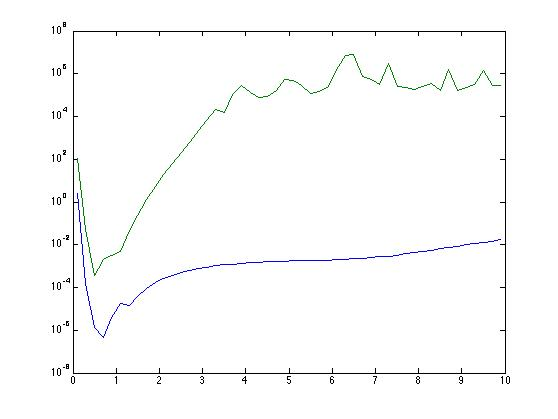
\includegraphics[scale=.4]{edp1_169_imq.jpg}
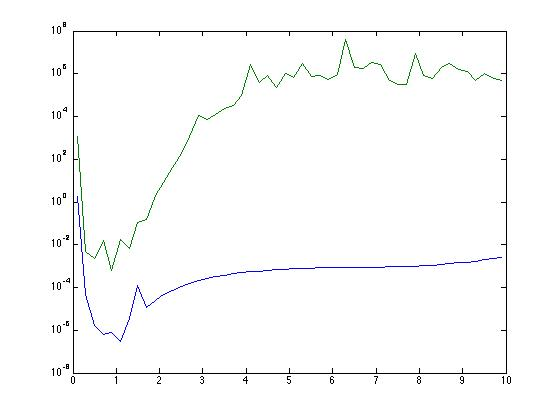
\includegraphics[scale=.4]{edp1_289_imq.jpg}
\caption{EDP1. IMQ. ECM y función coste.N=169 (izquierda) y N=289 (derecha).}
\end{figure}

\begin{figure}[H]
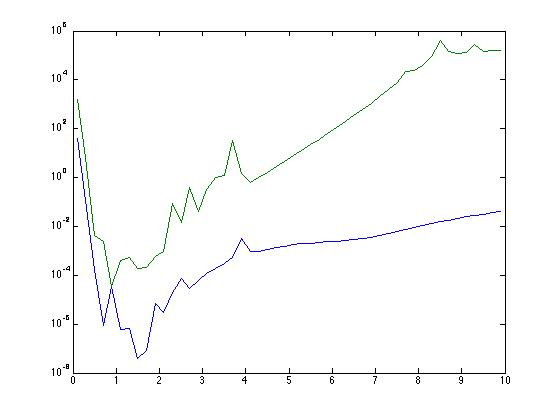
\includegraphics[scale=.4]{edp1_169_gaussiana.jpg}
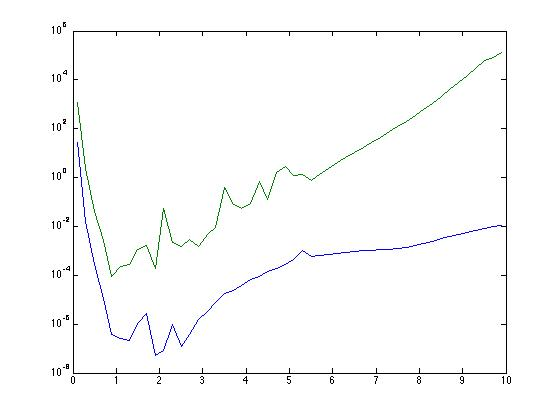
\includegraphics[scale=.4]{edp1_289_gaussiana.jpg}
\caption{EDP1. Gaussianas. ECM y función coste.N=169 (izquierda) y N=289 (derecha).}
\end{figure}
 \begin{table}
 \begin{center}
 \caption{Elección del parámetro de forma para la tercera EDP.}
 \begin{tabular}{|c|c|c|c|c|}
 \hline
  & \multicolumn{2}{|c|}{IMQ} & \multicolumn{2}{|c|}{Gaussiana}\\
  \hline
  $N$& 169 & 289 & 169 & 289 \\
  \hline
  $\epsilon$ óptimo & 0.7 & 1.1 & 1.5 &2.5  \\
  ECM($\epsilon$) &7.0968e-05 & 1.3715e-04& 5.6626e-05 &3.0003e-05 \\
  Estimación $\bar{\epsilon}$ & 0.5 & 0.9& 1.3 & 1.9 \\
  Coste & 2.5875e-01&8.5797e-02 & 6.4281e-02&2.1869e-01 \\
  ECM($\bar{\epsilon}$) &4.4364e-04 &5.1954e-04 &8.7362e-05 &3.7699e-05 \\
  \hline
 
 \end{tabular}
 \end{center}
 \end{table}
 \begin{figure}
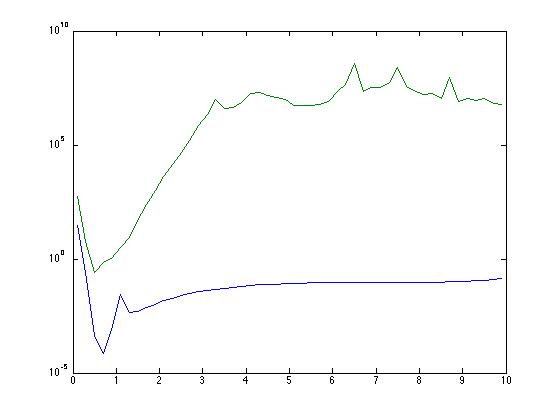
\includegraphics[scale=.4]{edp3_169_imq.jpg}
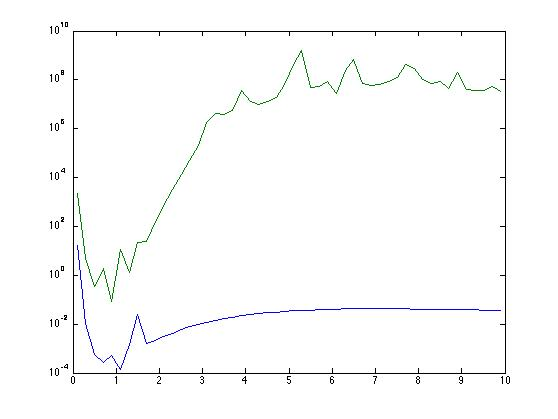
\includegraphics[scale=.4]{edp3_289_imq.jpg}
\caption{EDP3. IMQ. ECM y función coste. N=169 (izquierda) y N=289 (derecha).}
\end{figure}

\begin{figure}
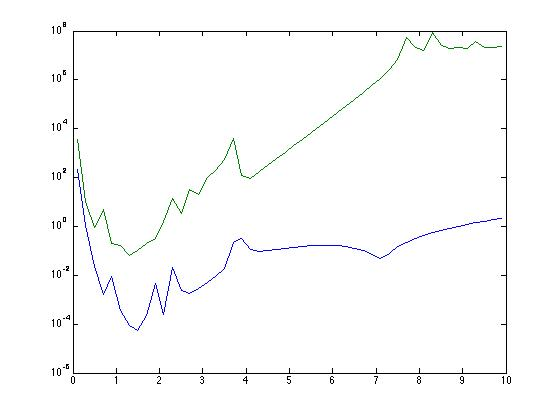
\includegraphics[scale=.4]{edp3_169_gaussiana.jpg}
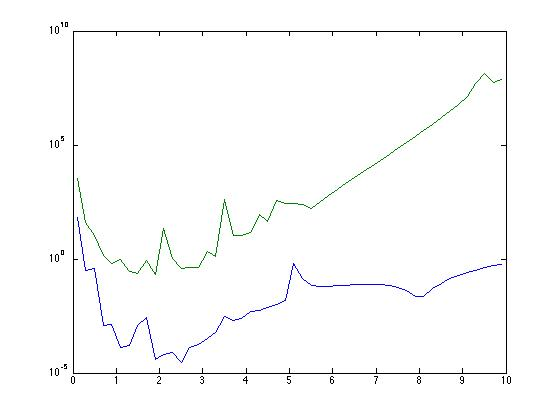
\includegraphics[scale=.4]{edp3_289_gaussiana.jpg}
\caption{EDP3. IMQ. Gaussianas y función coste.N=169 (izquierda) y N=289 (derecha).}
\end{figure}
\end{document}